\section{Inter-Process Communication}
Inter-process Communication (IPC) is a term describing communication between two processes through a shared interface. There are a number of variations of IPC. In operating systems like Unix and Windows there are a mechanisms for local IPC such as files, sockets, pipes, shared memory and semaphores. 
Inter-process communication using files is simply done by two processes reading and writing to one or more files. Pipes are a way of directing the output of one program to the input of another program. A variation of pipes are named pipes, also called FIFO (first in first out) which are system persistent pipes, often represented as files \cite{Lewandowski97interprocesscommunication}. Sockets are software abstractions to create a bidirectional channel between processes. They come in two variations, datagram sockets and stream sockets. Datagram sockets are faster than stream sockets but less reliable \cite{Lewandowski97interprocesscommunication}. Shared memory allows two processes to access the same memory and semaphores are used to signal availability of a resource between processes to avoid information loss, so called race conditions, while writing to the same block of memory from two different processes.

For communication between applications there are Inter-process communication implementations supporting communication with applications running on remote computers through interfaces of a higher abstraction than those for local IPC. These can also be used locally but the abstractions come at a cost in resources.

Remote IPC can be done in two ways unicast and multicast. Unicast is when the communication is sent from one entity and received by another entity. An example of unicast remote IPC is Remote Procedure Calls, RPC. Multicast is when the communication is sent from one entity and received by a group of entities. An example of multicast IPC is message passing which is used by the MediaSense platform to communicate between nodes over the Internet.

\subsection{Message Passing}
Message passing performs IPC by sending and receiving messages. Received messages are placed in a queue and are handled asynchronously.
The messages contain data which is used to determine the action or response. This allows the receiver to prioritize some messages. Message passing provides few abstractions for the developer and requires the data to be marshalled before sending messages and unmarshalled before receiving messages. 

The Message Passing Interface, MPI \cite{mpi3stand}, is one such standardized message passing implementation. Sending and receiving operations in MPI can be either blocking or non-blocking. Blocking send and receive operations wait for the application buffer to be free for reuse before returning to prevent race conditions, while non-blocking messages allow the process to proceed as soon as possible.

\subsection{Remote Procedure Calls}
Remote Procedure Calls (RPC) are a form of IPC that allow one process to invoke a callable unit \cite{Eac} located in another logical or physical space. Usage of RPC makes it possible to both interact with programs running on the same physical memory and with applications located within the same network. RPC is an abstraction built on top of message passing to enable calls to remote procedures as if they were made locally.
RPCs are unicast and synchronous, the sender waits for a response from the recipient before continuing the execution. Remote procedure calls are handled as if the calls were done locally, the calling process waits for a return value before proceeding, see Fig. \ref{rpc}.

Bruce Jay Nelson first defined Remote Procedure Calls as
\begin{quotation}
\centering
[...] the synchronous language-level transfer of control between programs in disjoint address spaces whose primary communication medium is a narrow channel.  \cite{Nelson:1981:RPC:910306}
\end{quotation}

\begin{figure}[ht]
		\centering	
		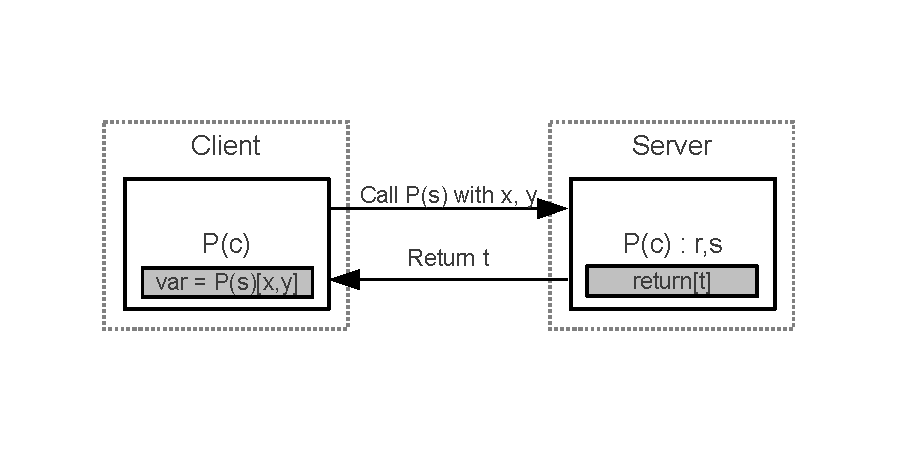
\includegraphics{part_2/remote_procedure_calls/rpc.pdf}
		\caption{Abstract of the events involved in remote procedure calls from a user perspective.
The procedure P(c) in the Client calls procedure P(s) located at the Server. The procedure P(s) receive two arguments r and s and return the value t which is stored in variable var back in the client.}
		\label{rpc}
\end{figure}

When using remote procedure calls, one process is considered the server and one the client. The client is the caller process and the server receives and handles the process and then returns the value. The client and server both have stubs, server-side stubs are called skeletons. Stubs are modules in charge of marshalling the calls, which means packing the parameters of the call in a way that allows them to be stored or transferred via Transmission Control Protocol (TCP) or User Datagram Protocol (UDP) \cite{rfc5531}. 
The events that occur when a client invokes a remote procedure call start with a call to the client's stub are shown in \ref{rpcflow}. The client stub receive the parameters from the local call and then marshalls. The marshalled data is then sent to the server by the the client's operating system. The server operating system receives the message and sends it to the skeleton. The skeleton unmarshalls the message  to obtain the parameters and invokes the local version of the procedure with the parameters. The server's procedure returns a value which is then sent to the skeleton. The skeleton then in turn marshalls the return value and sends the marshalled data back to the client. The client receives the message, the client stub unmarshalls the return value which then is sent back to the client's procedure \cite{Lewandowski97interprocesscommunication}. RPC implementations often is language specific. Some implementations, like XML-RPC and 
JSON-RPC use a common format for describing objects and can therefore be used cross-platform.

\begin{figure}[ht]
		\centering	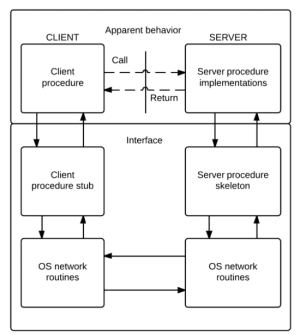
\includegraphics{part_2/remote_procedure_calls/Rpcflow300.png}
		\caption{The flow of a RPC}
		\label{rpcflow} 
\end{figure}

\subsection{Remote Method Invocation}
Remote method invocation (RMI) is a Java implementation of RPC with support for Java objects and allows entire objects to be passed and returned as parameters instead of only primitive data types. These objects can be dynamically loaded in the receiving Java Virtual Machine and can therefore be of an object type unknown to the receiver. RMI requires objects to be RemoteObjects, a remote object must implement a remote interface to support remote invocations. When a remote object is sent to another Java Virtual Machine it is sent as a remote stub to the receiving remote.
RMI relies on a registry to find other remote objects which have to be registered with a name. Other objects can then do a lookup on the registered name to get a reference to the Remote object. RMI registries can be shared between multiple JVMs on the same machine which facilitates communication from newly created processes to persistent ones.

\begin{figure}[ht]
	\centering
    	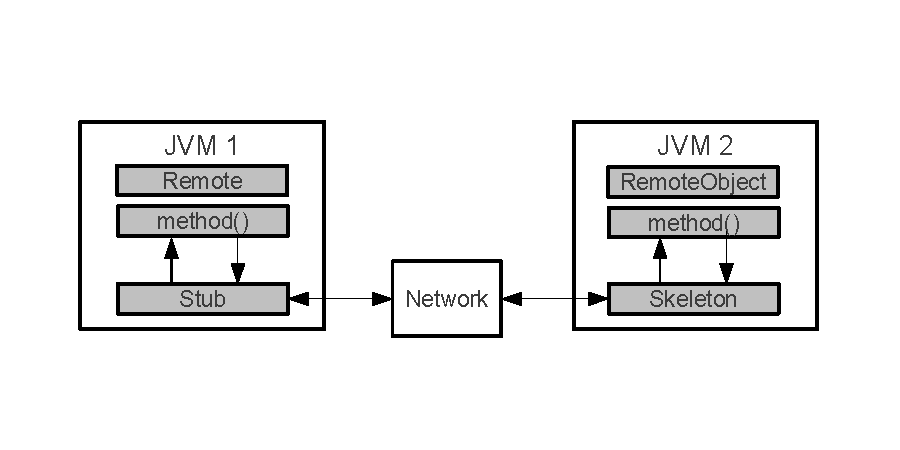
\includegraphics{part_2/remote_procedure_calls/rmi.pdf}
		\caption{The sequence of events in a method invocation with RMI.}
		\label{rmi} 
\end{figure}

\subsection{CORBA}
Common Object Request Broker Architecture is an object-oriented Remote Procedure Call mechanism. Corba is implemented in many different programming languages. This enables softwares written in different languages to communicate with each other. This is done with a language neutral API. CORBA uses an Object Request Broker which provides the mechanism required for distributed objects to communicate with each other. The Object Request Broker determines the location of target object, sends a request to that object and then returns a response back to the calling object. This communication is done over TCP/IP. However, in CORBA it is not possible to bind an Object Request Broker to a specific port. If the client is behind a firewall there is no option to change the port and use another port. This makes Corba firewall unfriendly.
